\section{Use case 2}\label{appendix:seapp_uc2}

In this use case we show how to confine an Ad library into an ad-hoc
process, with guarantees that it cannot abuse the access privileges
granted to the whole application sandbox by the user.  To do that, we
deliberately inject, in the same process the library is executed, a
malicious component (which is directly invoked by the library) that
tries to capture the location when the permission {\em
  ACCESS\textunderscore FINE\textunderscore LOCATION} is granted to
the app. The Ad library used is Unity Ads~\cite{seapp_unityads}, which
according to~\cite{seapp_ads_use} in 2020 was used by 11\% of apps
that show ads.
%
\begin{figure}[h]
  \centering
  \subfloat{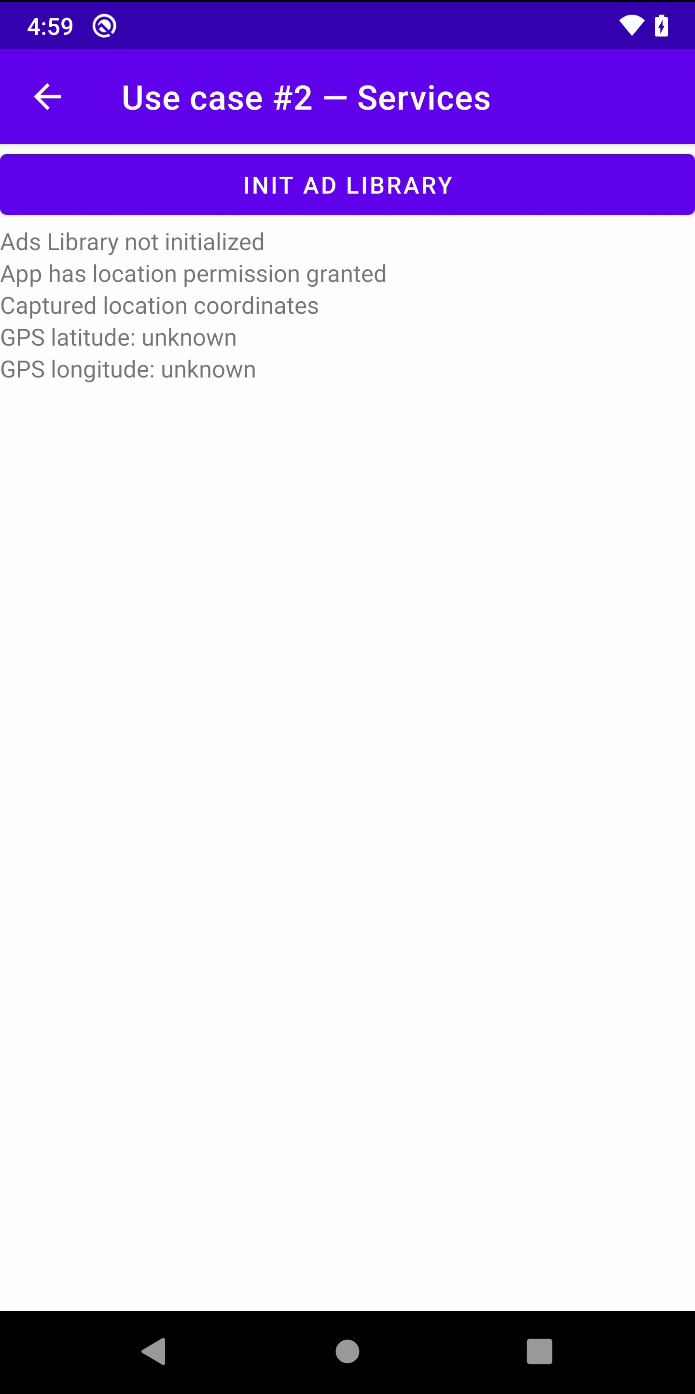
\includegraphics[width=0.3\textwidth]{chapters/seapp/figs/ae/uc21.png}}
  \hfill
  \subfloat{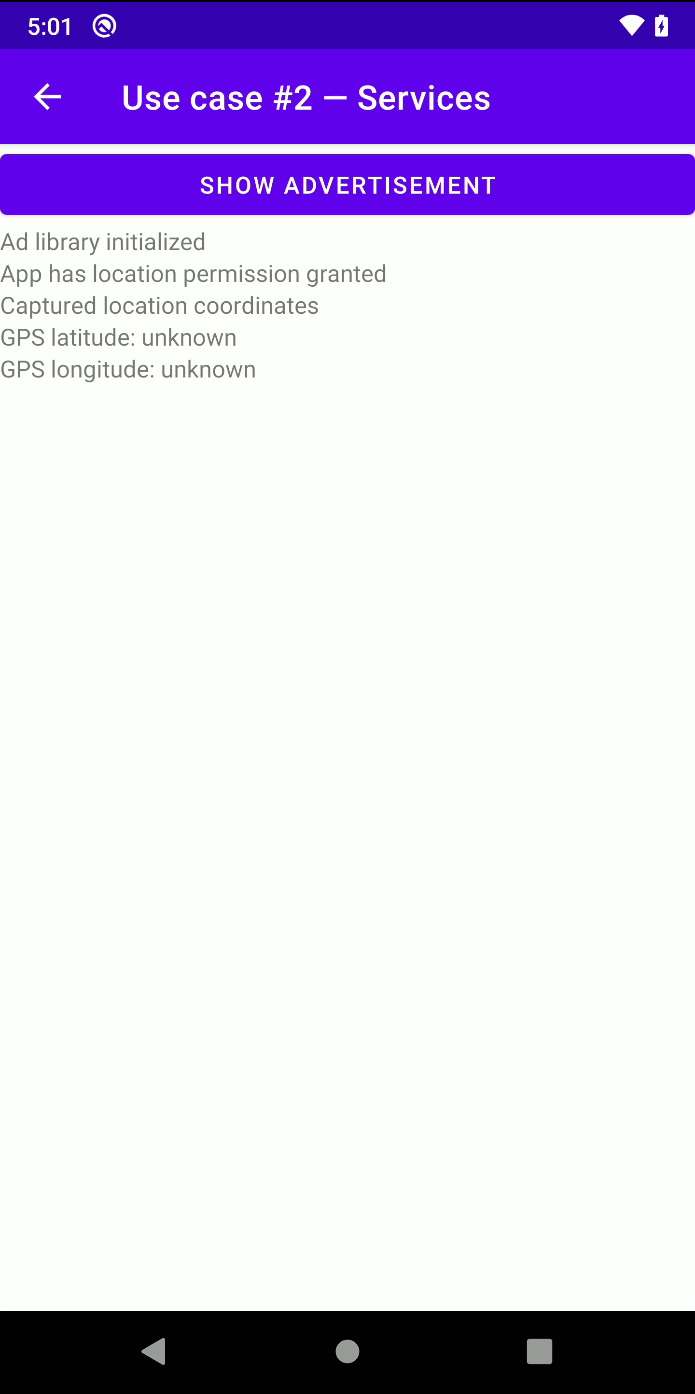
\includegraphics[width=0.3\textwidth]{chapters/seapp/figs/ae/uc22.png}}
  \hfill
  \subfloat{
\includegraphics[width=0.3\textwidth]{chapters/seapp/figs/ae/uc23.png}}
  \caption{\label{fig:seapp_uc2_views} Use case 2 views}
\end{figure}

In this case the library is invoked by {\em UseCase2Activity}
(Figure~\ref{fig:seapp_uc2_views}a), and according to line 3 of the
\seappcontexts, both the activity and the components created by the
library are executed by {\em Zygote} in a process labeled with {\tt
  ads\_d}.  To interact with the Ad library, {\em UseCase2Activity}
instances a {\tt UnityAdsListener}.  After the Ad initialization
(including the registration of the listener) and displaying the Ad to
the user (Figures~\ref{fig:seapp_uc2_views}b-c), the Ad framework
invokes the listener callback method {\tt onUnityAdsFinish}, which
executes the malicious routine {\tt captureLocation}. The routine
probes the app permissions; if {\em ACCESS\textunderscore
  FINE\textunderscore LOCATION} is granted to the app, the malicious
component retrieves through the \servicemanager a handle to the {\tt
  LocationManager}, and registers to it an asynchronous listener to
capture GPS location (Figure~\ref{fig:seapp_uc2_exploit}).

We show that when the policy module is enforced by \pap, the malicious
component cannot access the GPS coordinates. This is because the
component is executed in the same process of the library, which is
labeled with {\tt ads\textunderscore d}. If we look at the \sepolicy
(lines 43-50), {\tt ads\_d} is not granted access to the \sel type
{\tt location\textunderscore service}, so the malicious routine cannot
retrieve and therefore connect to the {\em location\textunderscore
  service}.  The following denial is written to the system log: {\em
  denied {\tt find} on {\tt location\textunderscore service} to the
  {\tt ads\textunderscore d} domain}
(Figure~\ref{fig:seapp_uc2_logcat1}). As a result, the malicious
component is terminated by the {\em ActivityTaskManager}
(Figure~\ref{fig:seapp_uc2_logcat2}).

The Ad library was included in the app as an {\em .aar}
archive. To confine it, no modification was necessary, only
the use of \manifest and \sepolicy was required.

\begin{figure}[h]
  \centering
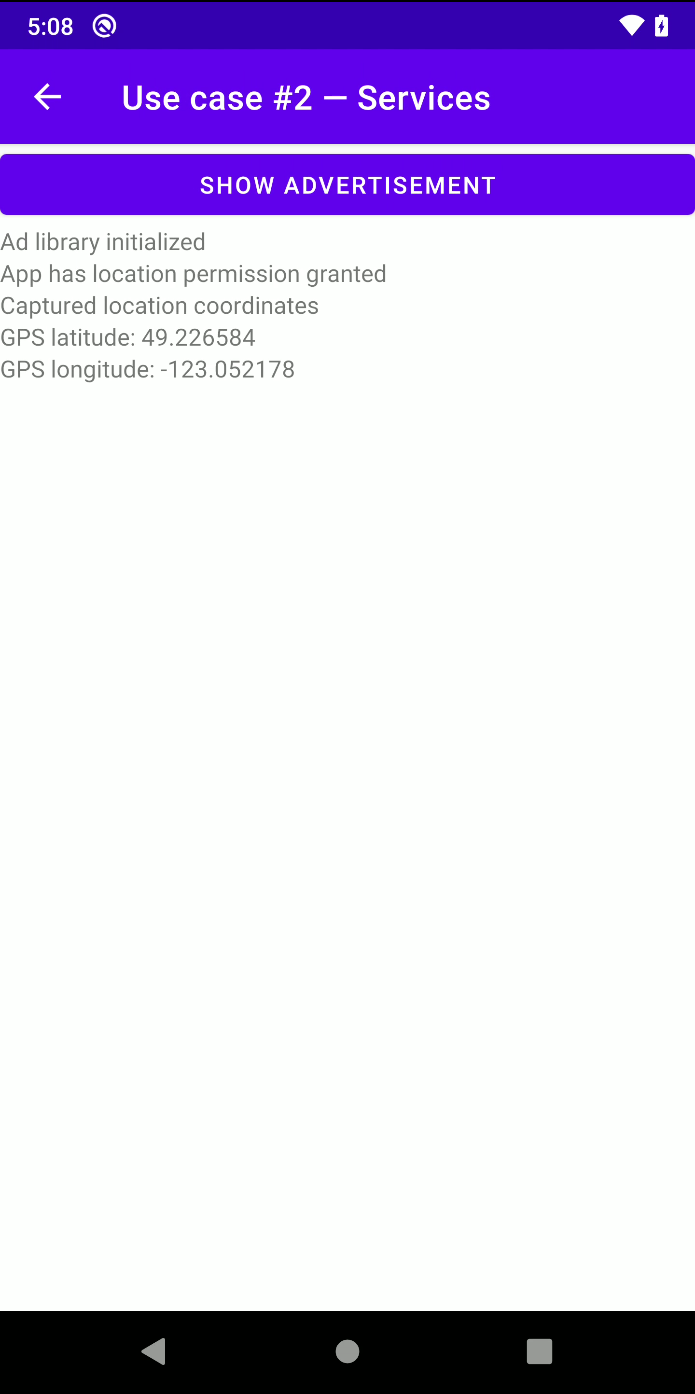
\includegraphics[width=0.29\textwidth]{chapters/seapp/figs/ae/uc24.png}
  \caption{\label{fig:seapp_uc2_exploit} Use case 2 exploit}  
\end{figure}  

\begin{figure}[h]
  \centering
  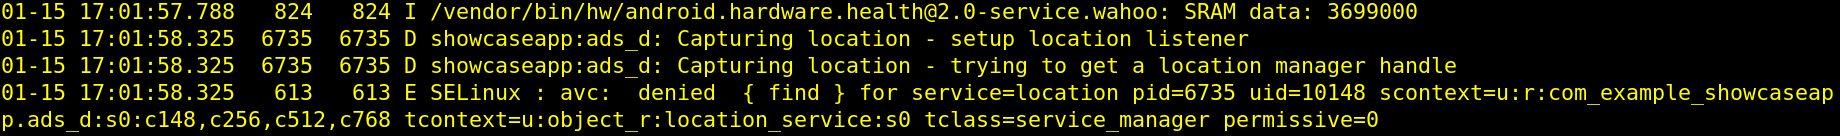
\includegraphics[width=\textwidth]{chapters/seapp/figs/ae/uc25.png}
  \caption{\label{fig:seapp_uc2_logcat1} Use case 2 logcat - \sel denial}  
\end{figure}      
\vspace{-1.3em}
\begin{figure}[h]
  \centering
  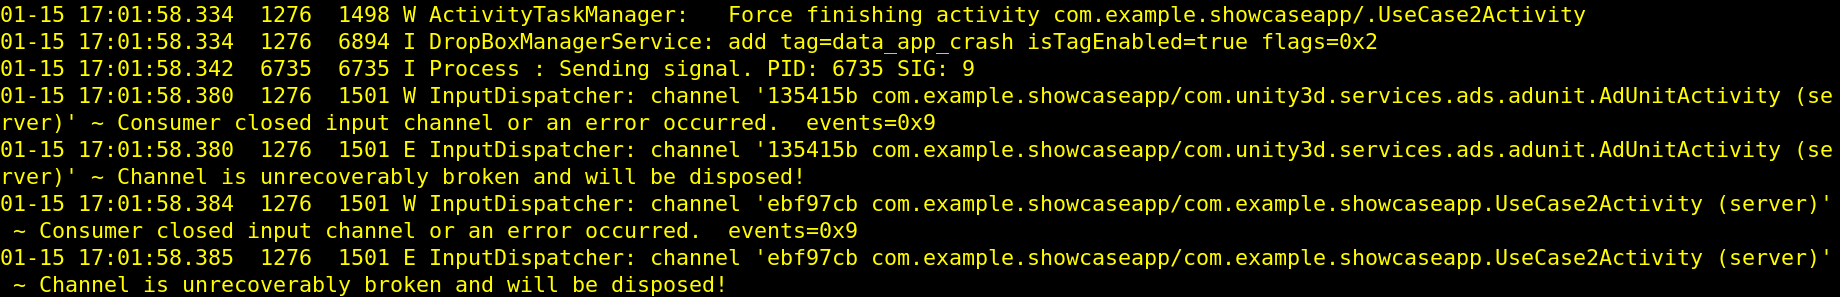
\includegraphics[width=\textwidth]{chapters/seapp/figs/ae/uc26.png}
  \caption{\label{fig:seapp_uc2_logcat2} Use case 2 logcat - Activity termination}  
\end{figure}      


%%% Local Variables: 
%%% mode: latex
%%% TeX-master: "../../../../main.tex"
%%% reftex-default-bibliography: "../../../../bib/biblio.bib"
%%% End:
